\documentclass[12pt]{article}

%%%%%%%%%%%%%%%%%%%%%%%%%%%%%%%%%%%%%%%%%%%%%%%%%%%%%%%%%%%%%%%%%%%%%%%%%%%%%%%%
%                           Package preset for homework
%%%%%%%%%%%%%%%%%%%%%%%%%%%%%%%%%%%%%%%%%%%%%%%%%%%%%%%%%%%%%%%%%%%%%%%%%%%%%%%%
% Miscellaneous
\usepackage[margin=1in]{geometry}
\usepackage[utf8]{inputenc}
\usepackage{indentfirst}
\usepackage{blindtext}
\usepackage{graphicx}
\usepackage{xr-hyper}
\usepackage{hyperref}
\usepackage{enumitem}
\usepackage{color}
\usepackage{float}
% Math
\usepackage{latexsym}
\usepackage{amsfonts}
\usepackage{amssymb}
\usepackage{amsmath}
\usepackage{commath}
\usepackage{amsthm}
\usepackage{bbold}
\usepackage{bm}
% Physics
\usepackage{physics}
\usepackage{siunitx}
% Code typesetting
\usepackage{listings}
% Citation
\usepackage[authoryear]{natbib}
\usepackage{appendix}
\usepackage[capitalize]{cleveref}
% Title & name
\title{Homework}
\author{Tien Vo}
\date{\today}


%%%%%%%%%%%%%%%%%%%%%%%%%%%%%%%%%%%%%%%%%%%%%%%%%%%%%%%%%%%%%%%%%%%%%%%%%%%%%%%%
%                   User-defined commands and environments
%%%%%%%%%%%%%%%%%%%%%%%%%%%%%%%%%%%%%%%%%%%%%%%%%%%%%%%%%%%%%%%%%%%%%%%%%%%%%%%%
%%% Misc
\sisetup{load-configurations=abbreviations}
\newcommand{\due}[1]{\date{Due: #1}}
\newcommand{\hint}{\textit{Hint}}
\let\oldt\t
\renewcommand{\t}[1]{\text{#1}}

%%% Bold sets & abbrv
\newcommand{\N}{\mathbb{N}}
\newcommand{\Z}{\mathbb{Z}}
\newcommand{\R}{\mathbb{R}}
\newcommand{\Q}{\mathbb{Q}}
\let\oldP\P
\renewcommand{\P}{\mathbb{P}}
\newcommand{\LL}{\mathcal{L}}
\newcommand{\FF}{\mathcal{F}}
\newcommand{\HH}{\mathcal{H}}
\newcommand{\NN}{\mathcal{N}}
\newcommand{\ZZ}{\mathcal{Z}}
\newcommand{\RN}[1]{\textup{\uppercase\expandafter{\romannumeral#1}}}
\newcommand{\ua}{\uparrow}
\newcommand{\da}{\downarrow}

%%% Unit vectors
\newcommand{\xhat}{\vb{\hat{x}}}
\newcommand{\yhat}{\vb{\hat{y}}}
\newcommand{\zhat}{\vb{\hat{z}}}
\newcommand{\nhat}{\vb{\hat{n}}}
\newcommand{\rhat}{\vb{\hat{r}}}
\newcommand{\phihat}{\bm{\hat{\phi}}}
\newcommand{\thetahat}{\bm{\hat{\theta}}}

%%% Other math stuff
\providecommand{\units}[1]{\,\ensuremath{\mathrm{#1}}\xspace}
% Set new style for problem
\newtheoremstyle{problemstyle}  % <name>
        {10pt}                   % <space above>
        {10pt}                   % <space below>
        {\normalfont}           % <body font>
        {}                      % <indent amount}
        {\bfseries\itshape}     % <theorem head font>
        {\normalfont\bfseries:} % <punctuation after theorem head>
        {.5em}                  % <space after theorem head>
        {}                      % <theorem head spec (can be left empty, 
                                % meaning `normal')>

% Set problem environment
\theoremstyle{problemstyle}
\newtheorem{problemenv}{Problem}[section]
\newenvironment{problem}[1]{%
  \renewcommand\theproblemenv{#1}%
  \problemenv
}{\endproblemenv}
% Set lemma environment
\newenvironment{lemma}[2][Lemma]{\begin{trivlist}
\item[\hskip \labelsep {\bfseries #1}\hskip \labelsep {\bfseries #2.}]}{\end{trivlist}}
% Set solution environment
\newenvironment{solution}{
    \begin{proof}[Solution]$ $\par\nobreak\ignorespaces
}{\end{proof}}
\numberwithin{equation}{problemenv}

%%% Page format
\setlength{\parindent}{0.5cm}
\setlength{\oddsidemargin}{0in}
\setlength{\textwidth}{6.5in}
\setlength{\textheight}{8.8in}
\setlength{\topmargin}{0in}
\setlength{\headheight}{18pt}

%%% Code environments
\definecolor{dkgreen}{rgb}{0,0.6,0}
\definecolor{gray}{rgb}{0.5,0.5,0.5}
\definecolor{mauve}{rgb}{0.58,0,0.82}
\lstset{frame=tb,
  language=Python,
  aboveskip=3mm,
  belowskip=3mm,
  showstringspaces=false,
  columns=flexible,
  basicstyle={\small\ttfamily},
  numbers=none,
  numberstyle=\tiny\color{gray},
  keywordstyle=\color{blue},
  commentstyle=\color{dkgreen},
  stringstyle=\color{mauve},
  breaklines=true,
  breakatwhitespace=true,
  tabsize=4
}
\lstset{
  language=Mathematica,
  numbers=left,
  numberstyle=\tiny\color{gray},
  numbersep=5pt,
  breaklines=true,
  captionpos={t},
  frame={lines},
  rulecolor=\color{black},
  framerule=0.5pt,
  columns=flexible,
  tabsize=2
}


\title{Homework 7: Phys 7320 (Spring 2022)}
\due{March 2nd, 2022}

\begin{document}
\maketitle
%%%%%%%%%%%%%%%%%%%%%%%%%%%%%%%%%%%%%%%%%%%%%%%%%%%%%%%%%%%%%%%%%%%%%%%%%%%%%%%
\begin{problem}{7.1}[A spaceship accelerating]
In this problem we will study the spacetime trajectory of an object that is
accelerating at a constant rate in its own (instantaneous) rest frame, and then
use it to think about an alien visit.

Consider a trajectory of a spaceship moving through space and time given by
\begin{equation}
    ct(\tau)=\frac{c^2}{a}\sinh\qty(\frac{a\tau}{c}),\qquad
    x(\tau)=\frac{c^2}{a}\qty[\cosh\qty(\frac{a\tau}{c})-1],
\end{equation}
where $\tau$ is the proper time of the spaceship, $c$ is the speed of light, $a$
is a constant that will turn out to be the acceleration of the ship in its own
frame, and $t$ and $x$ are coordinates in an inertial reference frame. Consider
only one-dimensional motion, so we can ignore $y$ and $z$. We see that at
$\tau=0$ the ship starts out at the spacetime origin $x=t=0$.

(a) Calculate the components of the four-velocity $U^\mu=dx^\mu/d\tau$ for the
spaceship. Using $U^\mu=(c\gamma,\gamma u)$, identify $\gamma$ and $u$ as
functions of $\tau$. Then invert the relation $t(\tau)$ and find $u$ s a
function of $t$. Find and discuss the limits of $u(t)$ for small $t$ and for
$t\to\infty$.

(b) The ship is accelerating, so it does not define an inertial frame. However,
at any moment in proper time there is an instantaneous rest frame moving with
the same velocity as the ship at that moment. For the proper time $\tau_0$, find
the Lorentz transformation bringing the spaceship momentarily to rest, using the
hyperbolic (rapidity) form.

(c) Find the components of the four-acceleration $\alpha^\mu=dU^\mu/d\tau$ in
the inertial frame for general proper times, and then at $\tau=\tau_0$ use the
Lorentz transformation you found in the last part to find the four-acceleration
in the instantaneous rest frame, thus showing that $a$ is indeed the magnitude
of the acceleration experienced by the spaceship in its own frame.

(d) Aliens are traveling from Proxima Centauri to the Earth by uniformly
accelerating their spaceship for half the trip, and then uniformly decelerating
with the same magnitude acceleration for the second half of the trip. What is
the elapsed time of the total one-way trip for the aliens on the spaceship, and
for observers on the Earth? (For the sake of the problem, pretend Earth and
Proxima are in the same stationary, inertial reference frame.) Use the
interstellar distance of $d=4.25$ light years and an acceleration of $8g$ (which
our bodies would have a hard time with, but these are tough aliens).
\begin{solution}
(a) By definition, we differentiate
\begin{equation}
    U^0=\frac{d(ct)}{d\tau}
    =c\cosh\qty(\frac{a\tau}{c}),\qquad\text{and}
    \qquad
    U^1=\frac{dx}{d\tau}=c\sinh\qty(\frac{a\tau}{c}).
\end{equation}
Then it follows that
\begin{equation}
    \gamma=\cosh\qty(\frac{a\tau}{c}),\qquad\t{and}\qquad
    u=c\tanh\qty(\frac{a\tau}{c})
    =c\frac{\sinh\qty(a\tau/c)}{\sqrt{1+\sinh^2\qty(a\tau/c)}}.
\end{equation}
Inverting $t(\tau)$, we get
\begin{equation}
    \tau(t)=\frac{c}{a}\sinh^{-1}\qty(\frac{at}{c}).
\end{equation}
Plugging this into the previous result, we obtain
\begin{equation}
    u(t)=\frac{at}{\sqrt{1+a^2t^2/c^2}}.
\end{equation}
Below we plot $u(t)$
\begin{center}
    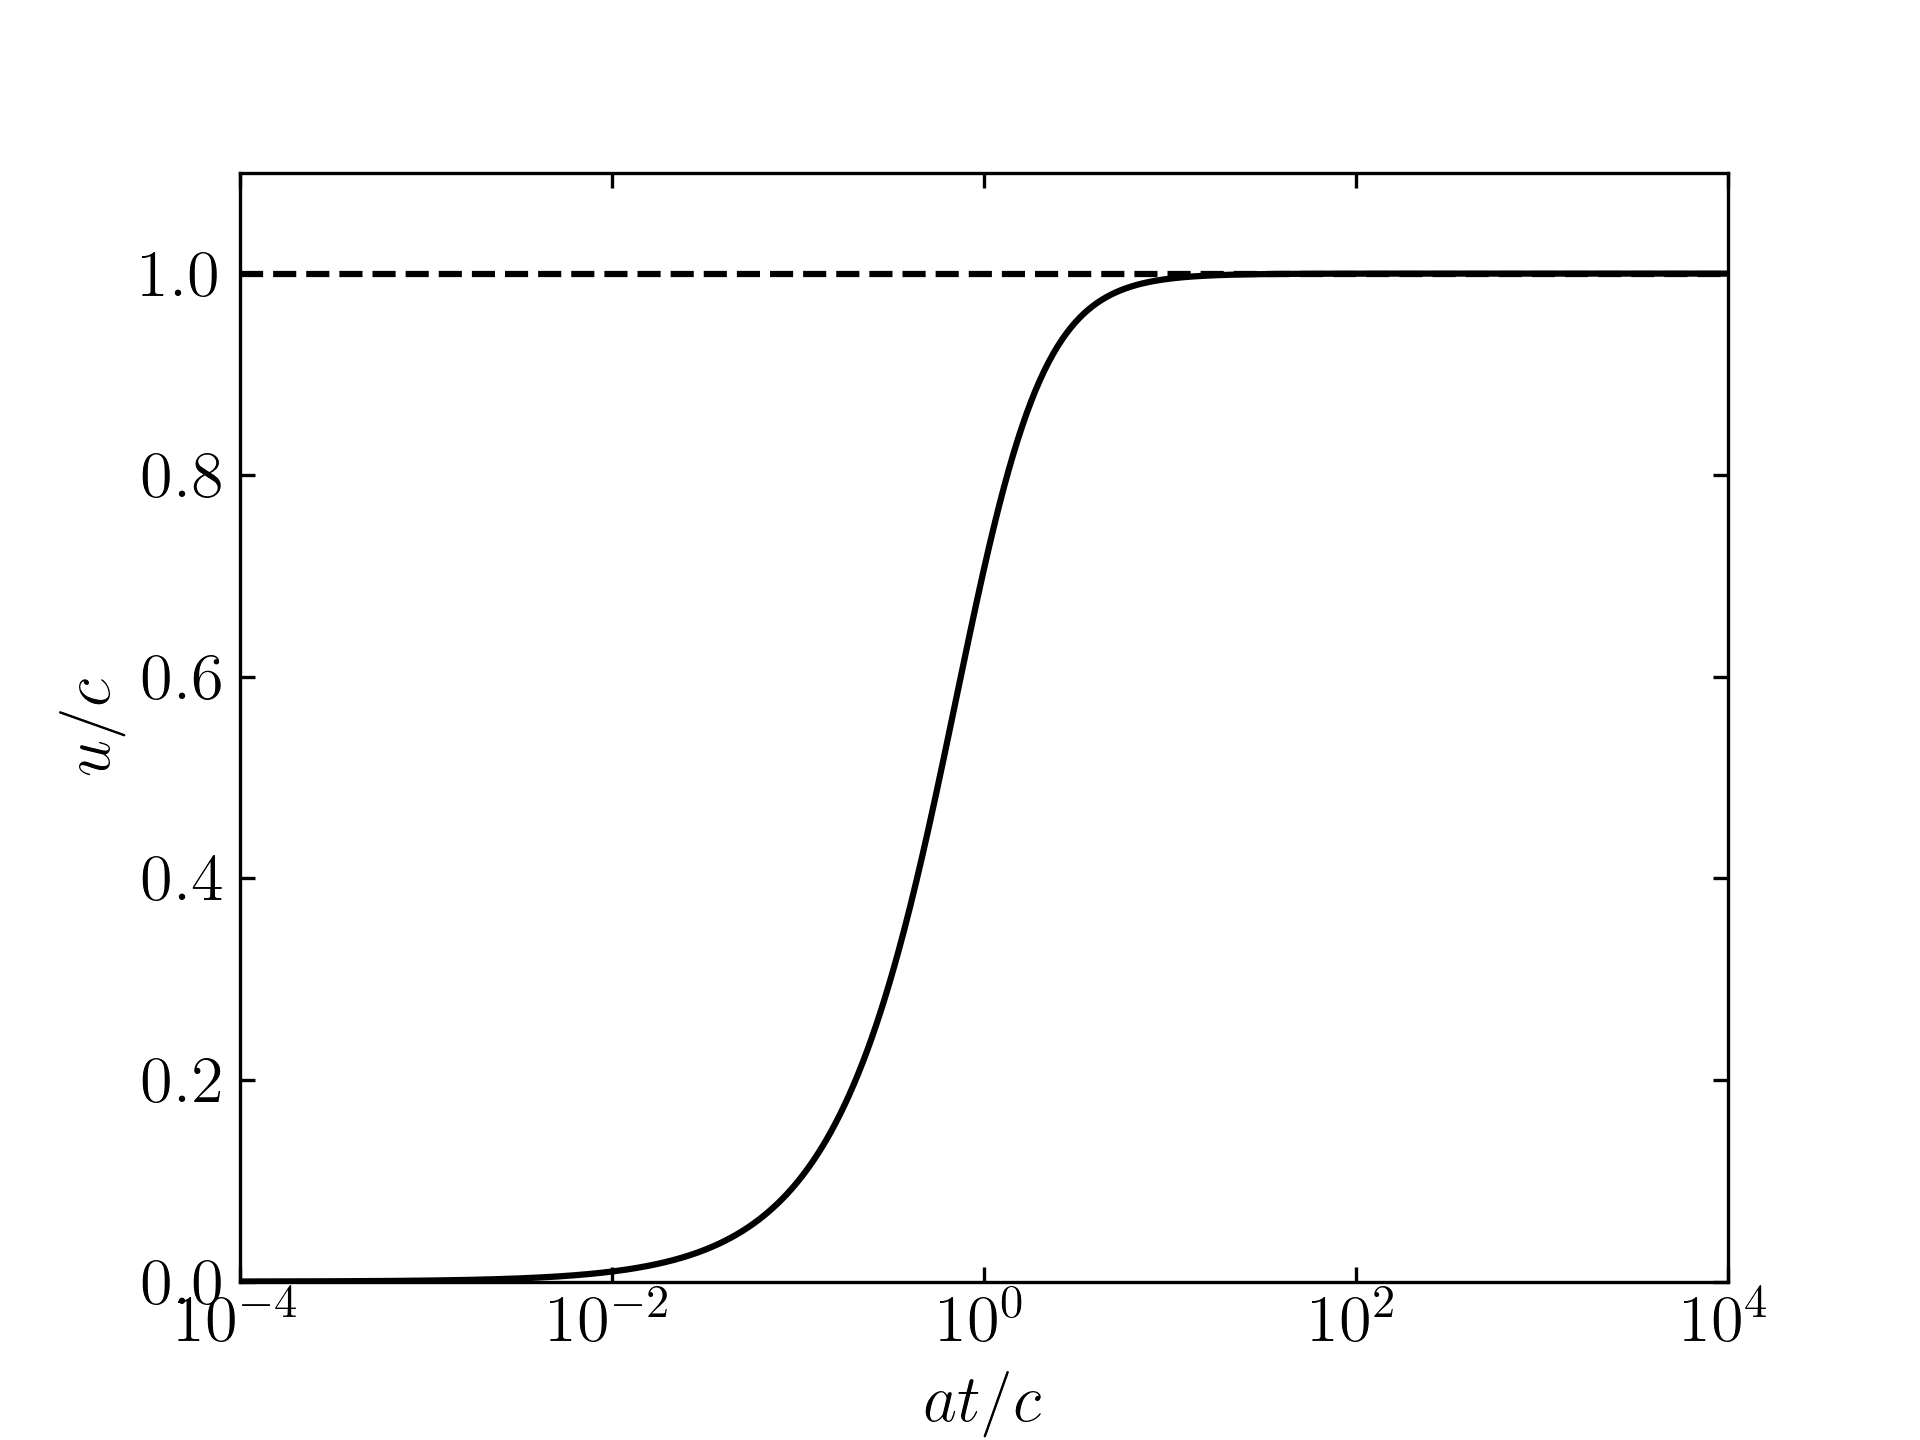
\includegraphics[width=0.7\textwidth]{p1a.png} 
\end{center}
Thus, $u=0$ at small $t$ and approaches $c$ asymtotically at $\infty$. This
means the spaceship accelerates from rest and reaches monotonically increasing
velocity, but never past the speed of light.

(b) Note that in hyperbolic form, $\zeta_0=a\tau_0/c$ is the rapidity. Thus, the
Lorentz transformation
\begin{equation}
    L(\tau_0)=\mqty(\cosh\zeta_0&-\sinh\zeta_0\\-\sinh\zeta_0&\cosh\zeta_0), 
\end{equation}
brings the spaceship momentarily to rest.

(c) By definition,
\begin{equation}
    \alpha^0=a\sinh\qty(\frac{a\tau}{c}),\qquad\t{and}\qquad
    \alpha^1=a\cosh\qty(\frac{a\tau}{c}).
\end{equation}
Under the Lorentz transformation, $\alpha^\mu$ transforms as
\begin{equation}
    \alpha'^\mu
    =a\mqty(\cosh\zeta_0&-\sinh\zeta_0\\-\sinh\zeta_0&\cosh\zeta_0)
    \mqty(\sinh\zeta_0\\\cosh\zeta_0)
    =a\delta_{\mu,1}
\end{equation}
Thus, the acceleration is truly $a$.

(d) In the Earth's (lab's) inertial frame, the accelerating/decelerating
proper time is $\tau_\pm$, determined by
\begin{equation}
    \frac{d}{2}=\pm\frac{c^2}{8g}\qty[\cosh\qty(\frac{8g\tau_\pm}{c})-1].
\end{equation}
Inverting this, we can write
\begin{equation}
    \sinh\qty(\frac{8g\tau_\pm}{c}) 
    =\frac{4dg}{c^2}\sqrt{1\pm\frac{c^2}{2dg}}.
\end{equation}
Plugging this back into $t(\tau)$,
\begin{equation}
    t_\t{total}=t(\tau_+)+t(\tau_-)
    =\frac{4d}{c}\qty[\sqrt{1+\frac{c^2}{2dg}}-\sqrt{1-\frac{c^2}{2dg}}]
    \approx 1.94\,\si{yr}.
\end{equation}
The total time measured by the aliens is
\begin{equation}
    \tau_\t{total}=\tau_++\tau_-
    =\frac{c}{8g}\qty[\sinh^{-1}\qty(\frac{4dg}{c^2}\sqrt{1+\frac{c^2}{2dg}})
    +\sinh^{-1}\qty(\frac{4dg}{c^2}\sqrt{1-\frac{c^2}{2dg}})]
    \approx0.86\,\si{yr},
\end{equation}
which is smaller than the inertial frame measurement as expected, since the
Proxima-Earth distance is Lorentz contracted in the spaceship frame.
\end{solution}
\end{problem}
\newpage
%%%%%%%%%%%%%%%%%%%%%%%%%%%%%%%%%%%%%%%%%%%%%%%%%%%%%%%%%%%%%%%%%%%%%%%%%%%%%%%    
%%%%%%%%%%%%%%%%%%%%%%%%%%%%%%%%%%%%%%%%%%%%%%%%%%%%%%%%%%%%%%%%%%%%%%%%%%%%%%%
\begin{problem}{7.2}[Equal mass elastic scattering]
Two particles $a$ and $b$, both with mass $m$, scatter elastically; label the
outgoing particles, also of mass $m$, as $c$ and $d$. Elastic scattering means
the \textit{total} 4-momentum before and after the collision is conserved. In
the center-of-mass frame, the scattering angle is $\theta'$. Show that the
scattering angle $\theta$ in a frame where one incident particle is at rest and
the other has energy $E$ (the ``lab frame'') is given by
\begin{equation}
    \cos^2\theta=\frac{\cos^2\theta'/2}{1-\frac{E-mc^2}{E+mc^2}\sin^2\theta'/2}.
\end{equation}
Comment on the nonrelativistic ($v\ll c$, $E\approx mc^2$) and ultrarelativistic
$(v\approx c,E\gg mc^2$) limits. To make the algebra less painful, work in units
where $c=1$, and restore it by dimensional analysis at the end.

\textit{Hint}: Consider 4-vector dot products $p_a\vdot p_b,p_b\vdot p_c$, and
$p_a\vdot p_c$. These are 4-scalars and therefore the same in all frames, that
is $p_a\vdot p_b=p_a'\vdot p_b'$ and so on. You will also want to recall the
relativistic relations between 3-momentum, mass and energy. Use the $p_a\vdot
p_b$ equation to solve for $E'$ in terms of $E$ and $m$, and the $p_b\vdot p_c$
equation to solve for $E_c$ in terms of $E,m$ and $\theta'$; also show the
useful relation
\begin{equation}
    E_c-m=\frac{E-m}{2}(1+\cos\theta'). 
\end{equation}
Then use $p_a\vdot p_c$ to find an expression for $\cos\theta$ that you can turn
into the answer needed.
\begin{solution}
First, with $p_a=\mqty(E&\vb{p})^T$ and $p_b=\mqty(m&\bm{0})^T$, where the
3-vectors are boldened, we can calculate $p_a\vdot p_b=mE$. By Lorentz
invariance,
\begin{equation}
    mE=p_a'\vdot p_b' 
    =\mqty(E'\\\vb{p}')\vdot\mqty(E'\\-\vb{p}')
    =E'^2+p'^2
    =2E'^2-m^2\Rightarrow
    E'^2=\frac{m(E+m)}{2}.
\end{equation}
Now, $p_b\vdot p_c=\mqty(m&\bm{0})^T\vdot\mqty(E_c&\vb{p}_c)^T=mE_c$, but also,
\begin{equation}
    mE_c=p_b'\vdot p_c'
    =\mqty(E'\\-\vb{p}')\vdot\mqty(E'\\\vb{p}_c')
    =E'^2+p'p_c'\cos\theta'.
\end{equation}
Now, note that the magnitude of the 4-vectors $p_b'$ and $p_c'$ is
$E'^2-p'^2=E'^2-p_c'^2=m^2$, since the mass are the same. So we can rewrite
\begin{equation}
    mE_c=E'^2+\qty(E'^2-m^2)\cos\theta'
    =m\frac{E+m}{2}+m\frac{E-m}{2}\cos\theta'.
\end{equation}
Thus,
\begin{equation}
    E_c-m=(E-m)\cos^2x, 
\end{equation}
where $x=\theta'/2$. Finally, we can calculate $p_a\vdot p_c
=EE_c-pp_c\cos\theta=E'^2-p'p_c'\cos\theta'=p_a'\vdot p_c'$. Plugging in
previous results,
\begin{equation}
    p\frac{p_c}{E_c}\cos\theta=(E+m)\qty(1-\frac{m}{E_c})
    =\qty(E+m)\frac{(E-m)}{E_c}\cos^2x
    =\frac{p^2}{E_c}\cos^2x.
\end{equation}
This leads to
\begin{align}
    \cos^2\theta
    &=\frac{p^2}{p_c^2}\cos^4x\notag\\
    &=\frac{(E^2-m^2)\cos^2x}{2m(E-m)+(E-m)^2(1-\sin^2x)}\notag\\
    &=\frac{(E^2-m^2)\cos^2x}{E^2-m^2-(E-m)^2\sin^2x}\notag\\
    &=\frac{\cos^2x}{1-\frac{(E-m)^2}{(E-m)(E+m)}\sin^2x}\notag\\
    &=\frac{\cos^2(\theta'/2)}{1-\frac{E-m}{E+m}\sin^2(\theta'/2)}\notag\\
    &=\frac{\cos^2(\theta'/2)}{1-\frac{E-mc^2}{E+mc^2}\sin^2(\theta'/2)},
\end{align}
where we have corrected for $c=1$ in the beginning.
\end{solution}
\end{problem}
\newpage
%%%%%%%%%%%%%%%%%%%%%%%%%%%%%%%%%%%%%%%%%%%%%%%%%%%%%%%%%%%%%%%%%%%%%%%%%%%%%%%
\end{document}
